

\section{INTRODUCTION} \label{sec:intr}


Knowledge graphs (KGs) have found widespread adoption in various Web applications, such as search~\cite{eder2012knowledge,paulheim2017knowledge}, recommendation~\cite{guo2020survey,li2020alimekg}, and question answering~\cite{yang2018hotpotqa,lewis2020retrieval}.  
Constructing large-scale KGs has been a very challenging task.
While we can extract new facts from scratch, aligning existing (incomplete) KGs together is practically necessary for real-world application scenarios. 
Over the past years, the problem of entity alignment~\cite{GCN-Align,tang2019bert-int}, or namely ontology mapping~\cite{li2008rimom} and schema matching~\cite{li2014rule}, has been a fundamental problem for \hhy{the Web research community}.

\begin{figure}[t]
\setlength{\abovecaptionskip}{-0.2mm}
\centering   
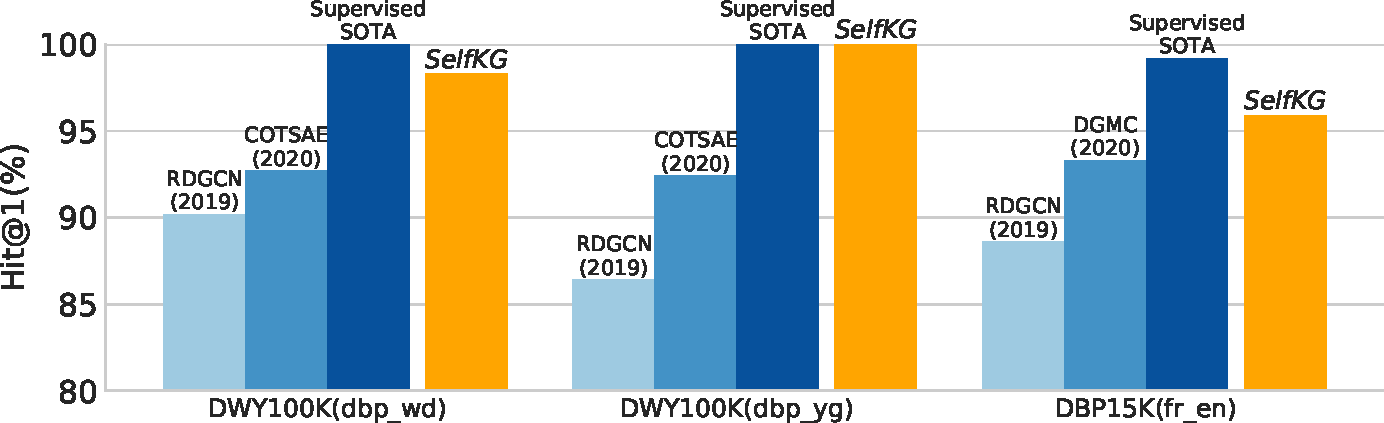
\includegraphics[width=\columnwidth]{img/intro.pdf}
\vspace{-1.5mm}
%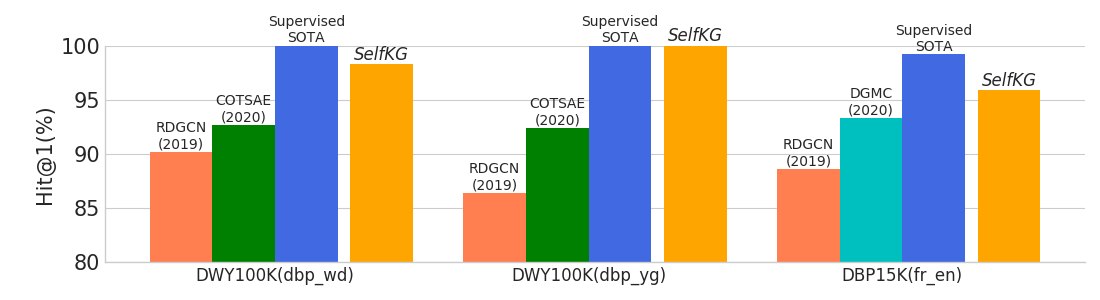
\includegraphics[width=1 \linewidth]{img/example.png}
\caption{Hit@1 on DWY100K and DBP15K for \solution (0\% of training labels) and SOTA supervised (100\% of training labels) entity alignment. \textmd{Without using any labels, the self-supervised \solution outperforms most of supervised models.}}
\label{fig:intro}
\vspace{-3.5mm}
\end{figure}

Recently, the representation learning-based alignment methods~\cite{MTransE,GCN-Align,CEAFF,tang2019bert-int,wu2019relation} have emerged as the mainstream solutions for entity alignment due to their superior flexibility and accuracy. 
However, their success relies heavily on the supervision provided by human labeling, which can be biased and arduously expensive to obtain for Web-scale KGs. 
In light of this fundamental challenge, we aim to explore the potential to align entities across KGs without label supervision (i.e., self-supervised entity alignment). 

To achieve this, we revisit the common process of the established supervised entity alignment approaches. 
%to identify the places where supervision is typically required.  
Conceptually, for each paired entities from two KGs, the goal of the existing learning objectives is to make them more similar to each other if they are actually the same entity (i.e., a positive pair), otherwise dissimilar if they are different entities (i.e., a negative pair). 
In the embedding space, this goal is pursued by pulling aligned entities closer and pushing different entities farther away.


We identify the parts where supervision is required in this process. At first place, the supervision serves to pull aligned entities closer.
Secondly, another issue arises is the procedure of generating label-aware negative pairs. 
For every entity in a KG, in the training its negative pairs are formed by randomly sampling entities from the other KG while excluding the groundtruth. 
%In fact, our analysis shows that a larger number of negative pairs used in training yields a theoretically guaranteed improvement.
If without supervision, it is likely that the implicitly aligned entities are sampled as negative pairs, thus spoiling the training (i.e., collision).


\vpara{Contributions.} 
We introduce the problem of self-supervised~\cite{liu2020self} entity alignment in KGs. 
To address it, we present the \solution framework, which does not rely on labeled entity pairs to align entities. 
It consists of three technical components: 1) relative similarity metric, 2) self-negative sampling, and 3) multiple negative queues. 

To get rid of label supervision, we theoretically develop the concept of relative similarity metric (RSM), which enables the self-supervised learning objective. 
The core idea of RSM is that instead of directly pulling the aligned entities closer in the embedding space, it attempts to push not-aligned negatives far away, thus avoiding the usage of the supervision of positive pairs. 
In a relative sense, the (implicitly) aligned entities can be considered to be dragged together when optimizing for RSM. 

By design, to address the dilemma between supervision with label-aware negative sampling and collision of false-negative samples without it, \solution further propose the self-negative sampling strategy, that is, for every entity in a KG, we form its negative pairs by directly sampling entities from the same KG. 
In other words, \solution solely relies on negative entity pairs that are randomly sampled from the input KGs . 
We theoretically show that this strategy remains effective for aligning entities across KGs. 


Finally, our theoretical analysis also shows that the self-supervised loss' error term decays faster as the number of negative samples increases, i.e., a large number of negative samples can benefit \solution. 
However, encoding massive negative samples on the fly is computationally very expensive. 
We address this by extending the MoCo technique~\cite{he2020momentum} to support two negative queues, each of which corresponds to the two KGs for alignments, ensuring an efficient increase of negative samples. 



Empirically, we conduct extensive experiments to demonstrate the premise of self-supervised entity alignment in KGs. 
We compare the proposed \solution method against 24 supervised and one unsupervised baselines on two widely-used entity alignment benchmarks datasets---DWY100K and DBP15K. 
The results suggest that \solution without using any labels can match or achieve comparable performance with the state-of-the-art supervised baselines (Cf.  Figure \ref{fig:intro}). 
This demonstrates the power of self-supervised learning for entity alignment as well as our design choices of \solution. 




























\hide{%%%%%%%%%%%%%%%%%%%%%%%%%%%%%%%%%%%%%%%%%%%%%%%%%%%%%%%%%%%%%%%%%%%%%%%%%%%%%%%%5



\section{INTRODUCTION} \label{sec:intr}

\begin{figure}[t]
\setlength{\abovecaptionskip}{-0.2mm}
\centering   
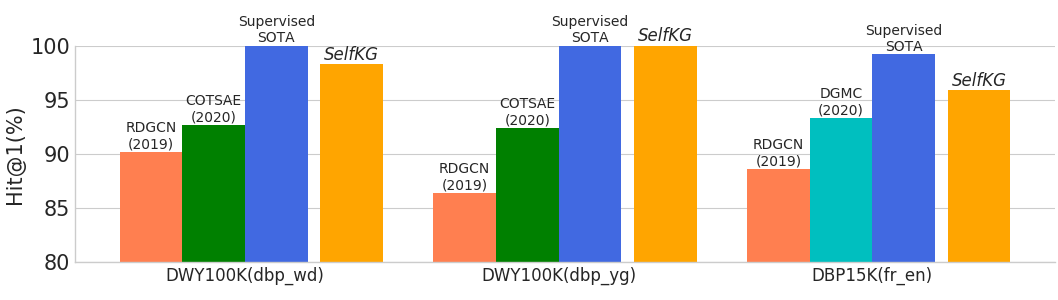
\includegraphics[width=\columnwidth]{img/example2.png}
%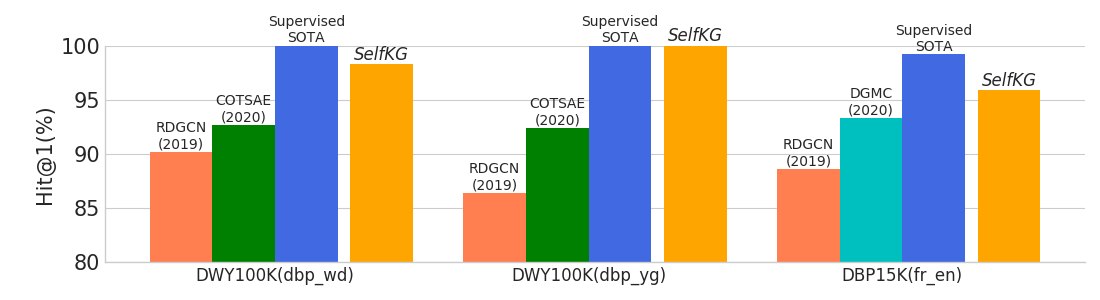
\includegraphics[width=1 \linewidth]{img/example.png}
\caption{Hit@1 on DWY100K and DBP15K(fr\_en) for \solution (0\% of training links) and SOTA supervised (100\% of training links) entity alignment. \textmd{Without using any labels for training, the self-supervised \solution outperforms most of the previous supervised models.}}
\label{fig:intro}
\vspace{-4mm}
\end{figure}


Knowledge graphs (KGs) have found widespread adoption in various Web applications, such as search~\cite{eder2012knowledge,paulheim2017knowledge}, recommendation~\cite{guo2020survey,li2020alimekg}, and question answering~\cite{yang2018hotpotqa,lewis2020retrieval}.  
Constructing large-scale KGs has been a challenging task.
While we can extract new facts from scratch,  aligning existing incomplete KGs to complement each other is practically necessary. 
Entity alignment~\cite{GCN-Align,tang2019bert-int}, or namely entity resolution, ontology mapping~\cite{li2008rimom}, and schema matching~\cite{li2014rule}, has been a fundamental problem for knowledge engineering, remaining far from resolved.

Recently, deep representation learning-based alignment methods~\cite{MTransE,GCN-Align,CEAFF,tang2019bert-int,wu2019relation} have emerged as the mainstream solutions due to their superior flexibility and accuracy. 
However, their success relies heavily on the supervision signals provided by human labeling, which can be biased and arduously expensive to obtain for Web-scale KGs. 
In light of this fundamental challenge, we aim to explore the potential to align entities across KGs without labels, that is, self-supervised entity alignment. 

To achieve that, we first revisit the common process of embedding-based entity alignment to identify the places where supervision is typically required.  
First, entities in different KGs, especially for the multi-lingual ones, lie in different data spaces, while entity alignment needs to be projected to the same embedding space, usually requiring supervision. 
Second, pulling aligned entities closer in the embedding space can not be done without knowing the anchors. 
Finally, knowing aligned entities would guarantee that we don't accidentally sample aligned ones as negatives, and thus avoid spoiling the training. 

\vpara{Contributions.} To get rid of supervision for knowledge alignment, we derive three insights corresponding to the three points aforementioned from self-supervised contrastive learning~\cite{liu2020self,he2020momentum}. 
First, we propose to leverage uni-space learning based on pre-trained language models for projecting entities from different sources into the same embedding space. 
Second, we develop the concept of relative similarity metric, that is, instead of directly pulling the aligned targets closer in the embedding space, we propose to push not-aligned negatives far away enough.
Third, 
to avoid accidental false-negative samples, 
we propose to sample negative samples from the source KG rather than from the target KG. 
Finally, we theoretically demonstrate the effectiveness of these strategies.

%To speed up the training, we design a negative queue that stores and provides masses of encoded negatives and a momentum update optimization strategy to stabilize the training.

\hhy{We are the first to introduce self-supervised learning into entity alignment to the best of our knowledge, and} in this work, we propose the self-supervised entity alignment model \solution, which is built upon the insights above. 
Specifically, to align entities without supervision,  we develop the following strategies for \solution. 
We leverage the idea of relative similarity metric to design the self-supervised contrastive loss without labeled alignments between two KGs. 
We further introduce self-negative sampling to provide the loss with guaranteed negative samples. 
Finally, 
recognizing the fact that the decay rate of the loss's error term relates to the number of negative samples,
we extend MoCo~\cite{he2020momentum} to support two negative queues, each of which corresponds to the source or the target KG during joint optimization, for an efficient increase of negative samples.


We evaluate the self-supervised \solution  with comparisons against 24 supervised and one unsupervised baselines. 
Experiments are conducted on two widely-used entity alignment benchmarks: DWY100K and DBP15K. 
The results suggest that \solution without using any labels can match or achieve comparable performance with the state-of-the-art supervised baselines (Cf.  Figure \ref{fig:intro}). 
This demonstrates the power of self-supervised learning for entity alignment as well as our design choices of \solution. 





}%%%%%%%%%%%%%%%%%%%%%%%%%%%%%%%%%%%%%%%%%%%%%%%%%%%%%%%%%%%%%%%%%%%%%%%%%%%%%%%%%%%%%%%%%%%%%%%%%%%%%%%%%%5